\documentclass[11pt]{article}
\usepackage[a4paper]{geometry}
\usepackage{algorithm}
\usepackage{algorithmic}
\usepackage{amssymb}
\usepackage{amsmath}
\usepackage{graphicx}
\usepackage{enumerate}
\usepackage{verbatim}

\title{\textbf{A Weight-Based Personalized Recommendation using
 Idiocentric and Collaborative Filtering}}
\date{}
\begin{document}

\maketitle
\section{Literature Survey}
\label{sec:literatureSurvey}
Recommendation systems have gained popularity in web based systems since the appearance of papers on collaborative filtering in the 1990s~\cite{resnick, shardanand, hill}.\\
\begin{itemize}
 \item ~\cite{resnick} explains the concept of collaborative filters. They introduce GroupLens as a system for collaborative filtering of netnews, to help people find articles they will like in the huge stream of available articles. They hypothesize that the users who have agreed on a certain aspect in the past will probably agree again.
 \item ~\cite{shardanand} describes a technique for making personalized recommendations to a user based on the similarities between the interest profile of that user and those of other users. They also test and compare four different algorithms for making recommendations using social information filtering.
 \item ~\cite{hill} presents an approach for collaborative recommendation where in the history of other users is used in the automation of a social method for informing choices to the user. Their results show that the communal history-of-use data can serve as a powerful resource for use in interfaces.
 \item ~\cite{konstan} determines the potential predictive utility for Usenet news. They develop a specially modified news browser that accepts ratings and displays predictions on a 1-5 scale. They compute the predictions using collaborative filtering techniques and compare the results with noncollaborative approaches.
 \item ~\cite{breese} describes several algorithms designed for collaborative filtering, including techniques based on correlation coefficients, vector-based similarity calculations, and statistical Bayesian methods. They compare the predictive accuracy of the various methods in a set of representative problem domains. Over the past decade, web systems have moved towards personalized recommendations for better user experience.
 \item ~\cite{durao} describes a tag-based system for personalized recommendation. They propose an approach which extends the basic similarity calculus with external factors such as tag popularity, tag representativeness and the affinity between user and tag.
 \item ~\cite{fabian} investigates user modeling strategies for inferring personal interest profiles from social web interactions. They analyze individual micro-blogging activities on twitter and compare different strategies for creating user profiles based on the twitter messages.
 \item ~\cite{andriy} presents a personalization algorithm for recommendation in folksonomies, which relies on hierarchical tag clusters.
 \item ~\cite{sarwar} explores and analyzes different item-based collaborative techniques. They look into different techiniques for computing item-item similarities and various techniques to obtain recommendations from them. Significant developments in learning using graph data has led to recent advances in recommendation techniques.
 \item ~\cite{toine} presents a recommendation algorithm that includes different types of contextual information. They model the browsing process of a user on a movie database by taking random walks over the contextual graph.
 \item ~\cite{ziyu} models personalized tag recommendation as a "query and ranking" problem. They also propose a novel graph-based ranking algorithm for interrelated multi-type objects.
\end{itemize}

\section{Detailed Design}

Figures \ref{componentDiagram} and \ref{activitydiagram} represents the component diagram and activity diagram for the recommendation system respectively.

\begin{figure}[htp]
\centering
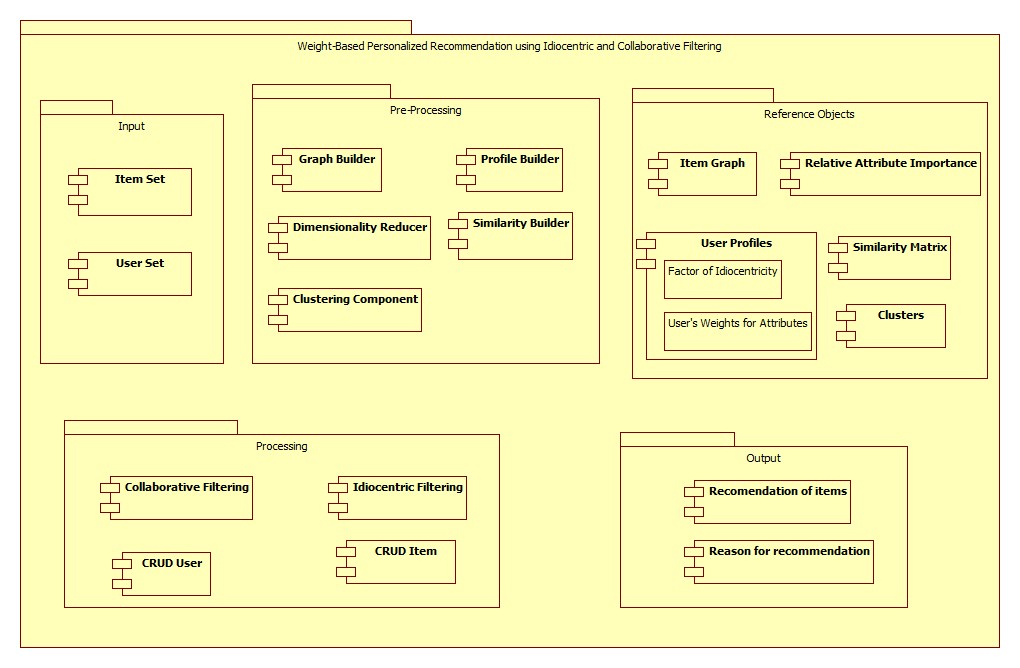
\includegraphics[scale=0.35]{Images/componentDiagram.jpg}
\caption{Component diagram for the Recommendation System}
\label{componentDiagram}
\end{figure}

\begin{figure}[htp]
\centering
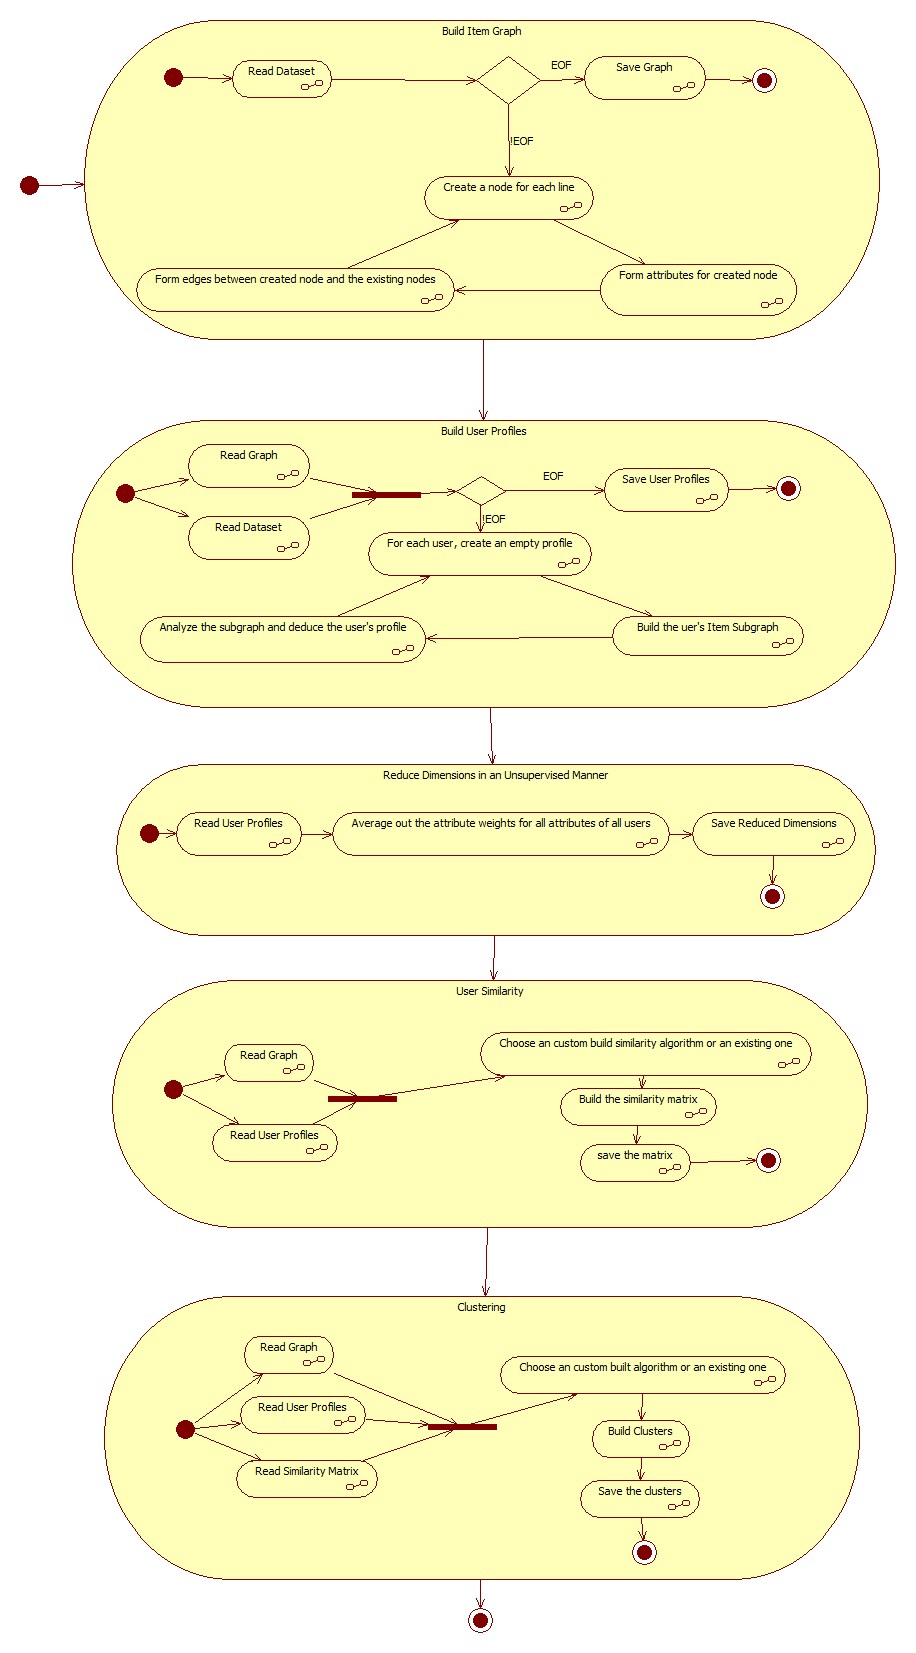
\includegraphics[scale=0.35]{Images/ActivityDiagram.jpg}
\caption{Activity diagram for the Recommendation System}
\label{activitydiagram}
\end{figure}

\section{Implementation}
\subsection{Read item dataset}
The input item dataset for the algorithm is a JSON file. The first line of the dataset gives the type information about all the attributes in the entire dataset. The JSON file is read into an in-memory object.\\

Eg:\\
\{
"rating": "float", \\
"genres": "string", \\
"filming\_locations": "string", \\
"rated": "string", \\
"language": "string", \\
"title": "string", \\
"country": "string", \\
"imdb\_id": "string", \\
"directors": "string", \\
"rating\_count": "integer"\}


\subsection{Build KeyValueNodes}
KeyValueNodes is a reverse-indexed associative array that we use to store details about items and the relationship among them.\\
Eg:\\
\{  

"directors": \{

\hspace{26 mm} "Stuart Gillard": [ "3354" ],

\hspace{26 mm} "Tobe Hooper": ["1911", "2294","2377","2937","3210"],

\hspace{26 mm} ...

\hspace{20 mm} \},

...
\\
\}

\subsubsection{Approach}
This subsection explains the approach that we use to build KeyValueNodes. The item dataset consists of both categorical and non-categorical data. The categorical data will be either string or boolean type (Eg: Director and Like, respectively). Non-categorical data includes all the numerical attributes. (Eg: rating, year, timestamp). Algorithms \ref{buidingkeyvaluenodes_1_algo} and \ref{buidingkeyvaluenodes_2_algo} depict the approach that we use to build KeyValueNodes.
\\
\\
\bf{Input:} set of items $I$ \\
\bf{Output:} $KeyValueNodes$
\begin{algorithm}
\label{buidingkeyvaluenodes_1_algo}
\caption{\bf for categorical data}
\begin{algorithmic}[1]
\STATE Initialize $KeyValueNodes$ to an empty associative array
\FORALL{items $i$ in $I$}
\FORALL{categorical attributes $attribute$ in $i$}
\FORALL{values $value$ that $attribute$ can take}
\STATE add $i$ to the $KeyValueNodes[attribute][value]$

\ENDFOR
\ENDFOR
\ENDFOR
\end{algorithmic}
\end{algorithm}
\\
\begin{algorithm}
\label{buidingkeyvaluenodes_2_algo}
\caption{for non-categorical data}
\begin{algorithmic}[1]
\STATE Initialize $D$ to an empty associative array

\FORALL{non-categorical attributes $attribute$ in the dataset}
  \STATE set D[$attribute$] to empty list
\ENDFOR

\FORALL{item $i$ in I}
    \FORALL{non-categorical attributes $attribute$ of $i$}
       \STATE D[attribute] $\leftarrow$ D[attribute] $\cup$ values taken by $attribute$ for $i$
    \ENDFOR
\ENDFOR

\STATE $clusters$ $\leftarrow$ empty associative array
\FORALL{$attribute$ in D}
  \STATE $cutpoints$ $\leftarrow$ $[]$
  \STATE sort D[$attribute$]
  \STATE $differences$ $\leftarrow$ list of differences between consecutive values of D[$attribute$]
  \STATE $avrg$ $\leftarrow$ average of $differences$
  \STATE populate $cutpoints$ with the indices for which the difference is greater than $avrg$
  \STATE populate $clusters[attribute]$ with list of values that fall between the consecutive indices
\ENDFOR

\FORALL{item $i$ in I}
  \FORALL{non-categorical attribute $attribute$ of $i$}
    \STATE clust $\leftarrow$ cluster that the value of $attribute$ belongs to
    \STATE add $i$ to the $KeyValueNodes[attribute][clust]$
  \ENDFOR
\ENDFOR
\end{algorithmic}
\end{algorithm}

\subsection{Generate user sequence}
\normalfont
The user dataset originally is the form of :
\begin{center}
$user-id : item-id : rating : epoch$ 
\end{center}

We convert this dataset to a JSON format in which we list all the users along with their item-id and corresponding rating in a chronological fashion.
Eg:\\
\{ \\
  "5988": [ 
  
\hspace{15 mm} ["587", "1"],

\hspace{15 mm} ["588", "3"],

\hspace{15 mm} ["3006", "4"],

\hspace{15 mm} ...

\hspace{8 mm} ],

...\\
\}

\normalmarginpar
\subsection{Build user profile}
A user is an entity who consumes an item. In this section,
we build a profile for each user. The user profile consists
of characteristic parameters of the user that quantifies his behaviour. In Algorithm \ref{buidinguserprofile_algo}, we explain the methodology to build user profiles with frequency based relative attribute importance.
 
\subsubsection{Frequency based relative attribute importance}
\begin{algorithm}
\label{buidinguserprofile_algo}
\caption{Building user profile}
\begin{algorithmic}[1]
\renewcommand{\algorithmicrequire}{\textbf{Input:}}
\renewcommand{\algorithmicensure}{\textbf{Output:}}
\REQUIRE $KeyValueNodes$
\ENSURE  $userProfiles$
\STATE Initialize $userProfiles$ to an empty associative array
\FORALL{users $u$}
\STATE $itemSequence \leftarrow$ items $u$ has consumed 
\FORALL{ attributes $attribute$ in $KeyValueNodes$}
\FORALL{ values $value$ in $KeyValueNodes[attribute]$}
\STATE  $n \leftarrow$   $ | itemSequence \cap KeyValueNodes |$
\STATE increment userProfiles[u][``weights``][attribute] by $^nC_2$
\ENDFOR
\ENDFOR
\ENDFOR
\end{algorithmic}
\end{algorithm}

\subsubsection{Range based normalization}
\begin{algorithm}
\label{buidingusernormalize_algo}
\caption{Range based normalization}
\begin{algorithmic}[1]
\renewcommand{\algorithmicrequire}{\textbf{Input:}}
\renewcommand{\algorithmicensure}{\textbf{Output:}}
\REQUIRE $userProfiles$
\ENSURE Range based normalization of $userProfiles$ 
\FORALL{$profile$ in $userProfiles$ }
\FORALL{ $attribute$ in $profile$}
\STATE  $userProfiles[profile][''weights``][attribute] \leftarrow$  $userProfiles[profile][''weights``][attribute] \times$ $|KeyValueNodes[attribute]|$
\ENDFOR
\ENDFOR

\FORALL{$profile$ in $userProfiles$ }
\STATE sumOfWeights $\leftarrow$ sum(userProfiles[profile]["weights"])
\FORALL{$attribute$ in $profile$}
\STATE userProfiles[profile]["weights"][attribute] $\leftarrow$ $\frac{userProfiles[profile]["weights"][attribute]}{sumOfWeights}$
\ENDFOR
\ENDFOR
\end{algorithmic}
\end{algorithm}

\subsection{Dimensionality reduction}
 In this section, we present an empirical approach to perform dimensionality reduction on the dataset. We observe the users' pattern in consuming the items and deduce the importance of an attribute. The importance of an attribute in the item dataset increases as number of users who give higher relative importance to that attribute increases. Hence, the importance of an attribute $a$ in the item set $I$ can be quantified as the mean relative importance of $a$, taken over all the users $u \in U$. In the previous section, we created a profile for each user. The characteristic parameter $w_{u_p}$ consists of relative weights of attributes for $u_p$. The relative importance of an attribute $a$ in the item set $I$ can be computed as follows:

\begin{equation}
weight_a = \frac{\sum_{u_p \in U} w_{u_p}[a]}{Number\ of\ Users} 
\end{equation}

\begin{figure}[htp]
\centering
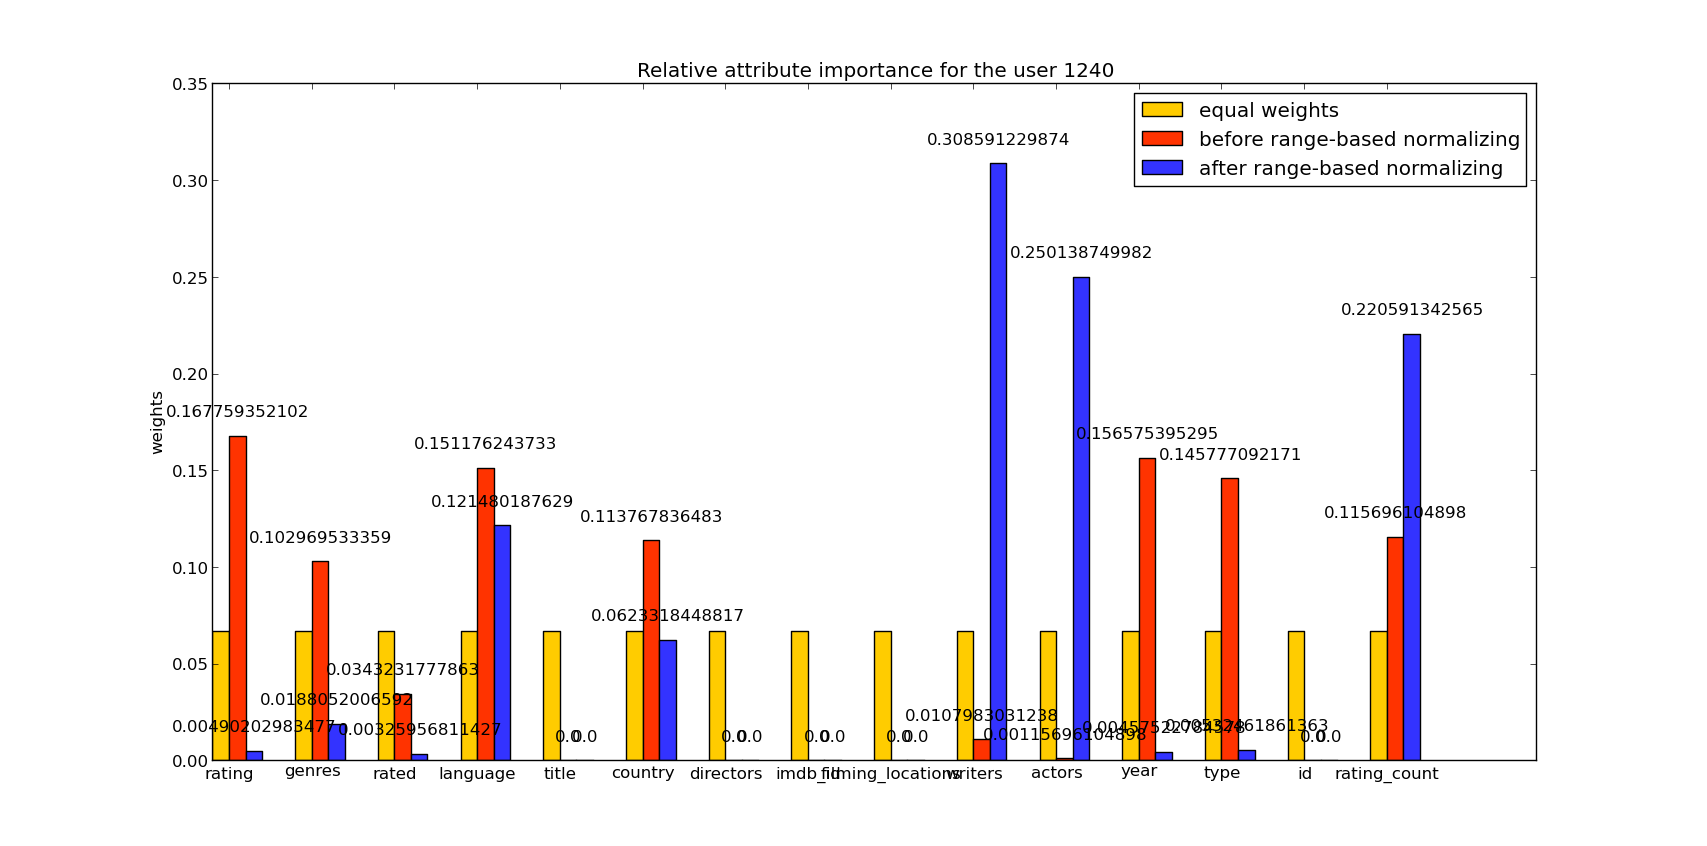
\includegraphics[scale=0.3]{Images/user1240new.png}
\caption{The figure indicates the relative attribute importance for the user 1240 before and after range based normalization.}
\label{attribRelFreq_items}
\end{figure}

\newpage
\bibliographystyle{plain}
\bibliography{references}

\end{document}
